
\subsection{Satellite vs Model Data} \label{subsec:satvsmod}




\begin{wrapfigure}[50]{r}{0.25\textwidth}

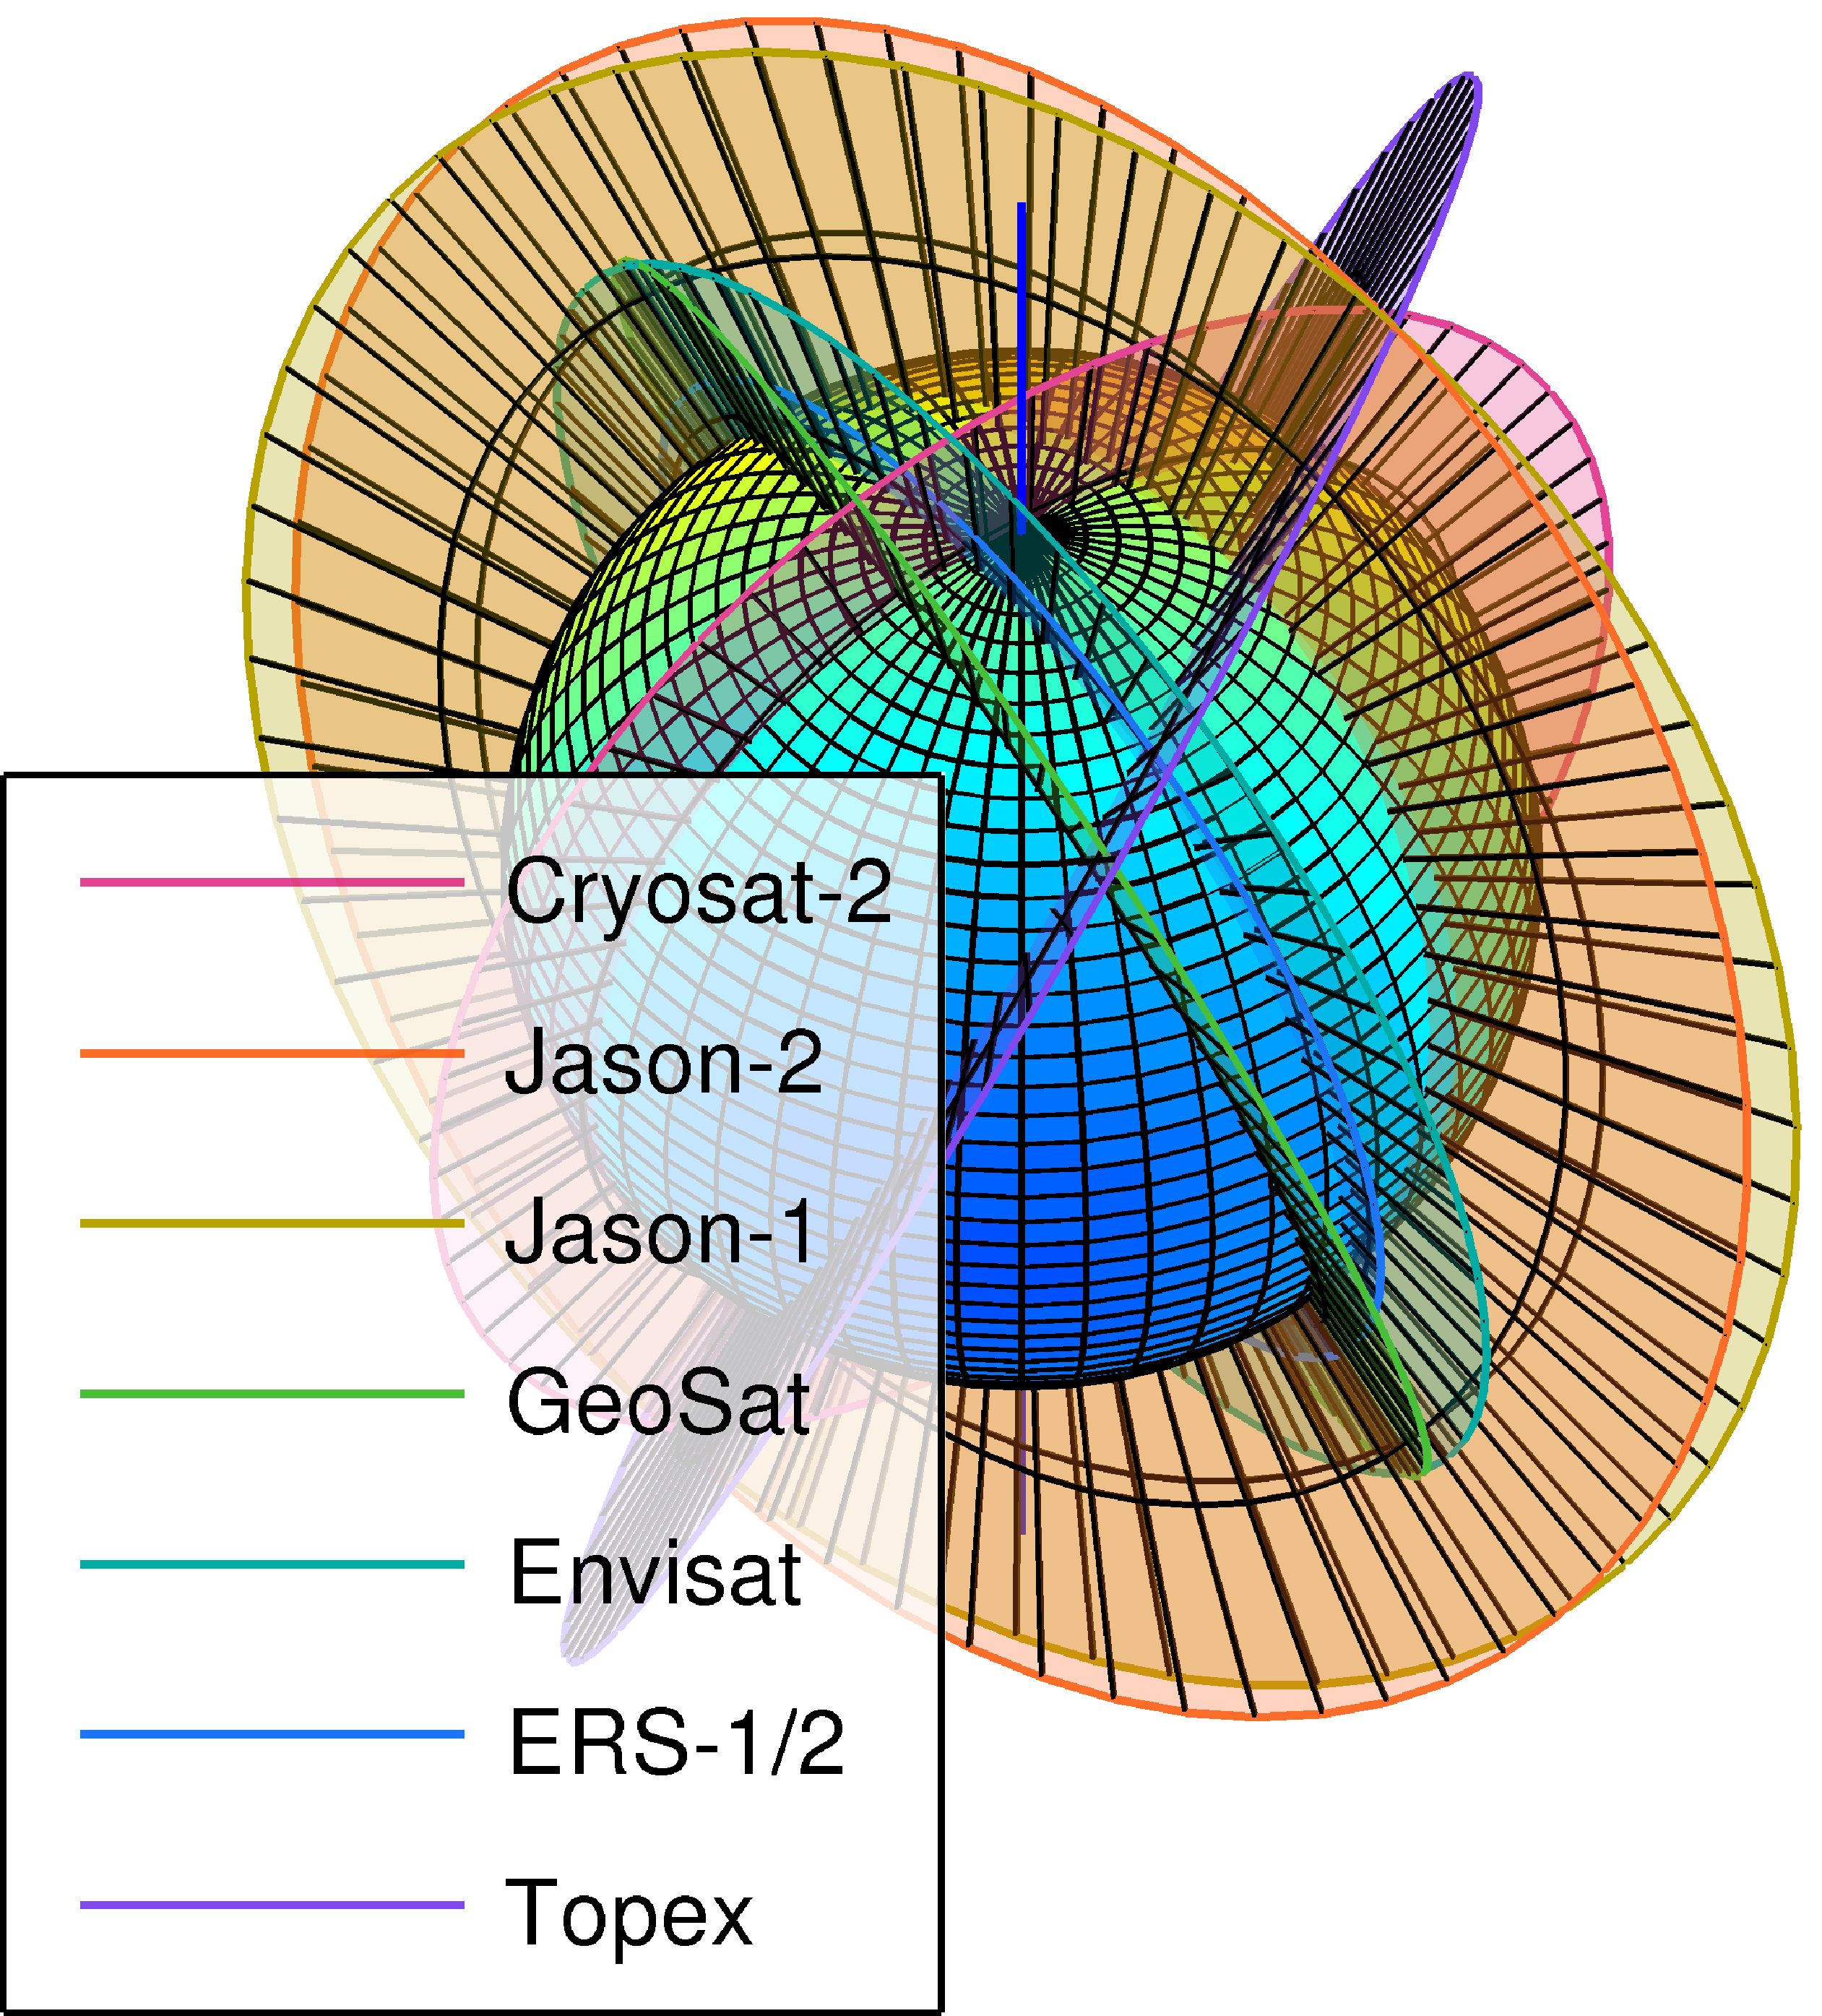
\includegraphics[width=.25\textwidth]{orbits3.pdf}

%\caption{Orbits for Aviso-relevant satellites.}
\end{wrapfigure}

\paragraph{Satellites}The latest Aviso SSH data from satellites features impressive accuracy, constancy and resolutions in both space and time. This is achieved
by collecting all of the data from all of the altimeter-equipped satellites available at any given moment for any given coordinate. This conglomerate of highly
inhomogeneous data is then subjected to state-of-the-art interpolation methods to produce a spatially and temporally coherent product. One satellite alone is
not sufficient to adequately resolve meso-scale variability globally. Take \eg the Topex/Poseidon satellite. It had a ground repeat track orbit of 10 days and
circled the earth in 112 minutes or $\approx 13$ times a day with a swath width of 5 km. Hence it drew $\approx 26$ 5 km-wide stripes onto the globe every day.
This pattern is then repeated after 10 days, which means that at the equator only $10 \times 26 \times 5=1300$km of the $2\pi \times 6371=40000$km get covered,
\ie $3.25\%$. At every $10d$ time step, on average, effectively
$40000/1300-5= 20$km are left blank in-between swaths on the equator. This is why, no matter how fine the resolution within the swath at one moment in time may
be, the spatial resolution is so coarse.



\begin{wrapfigure}[20]{r}{0.6\textwidth}
\vspace{-8mm}
  \begin{center}
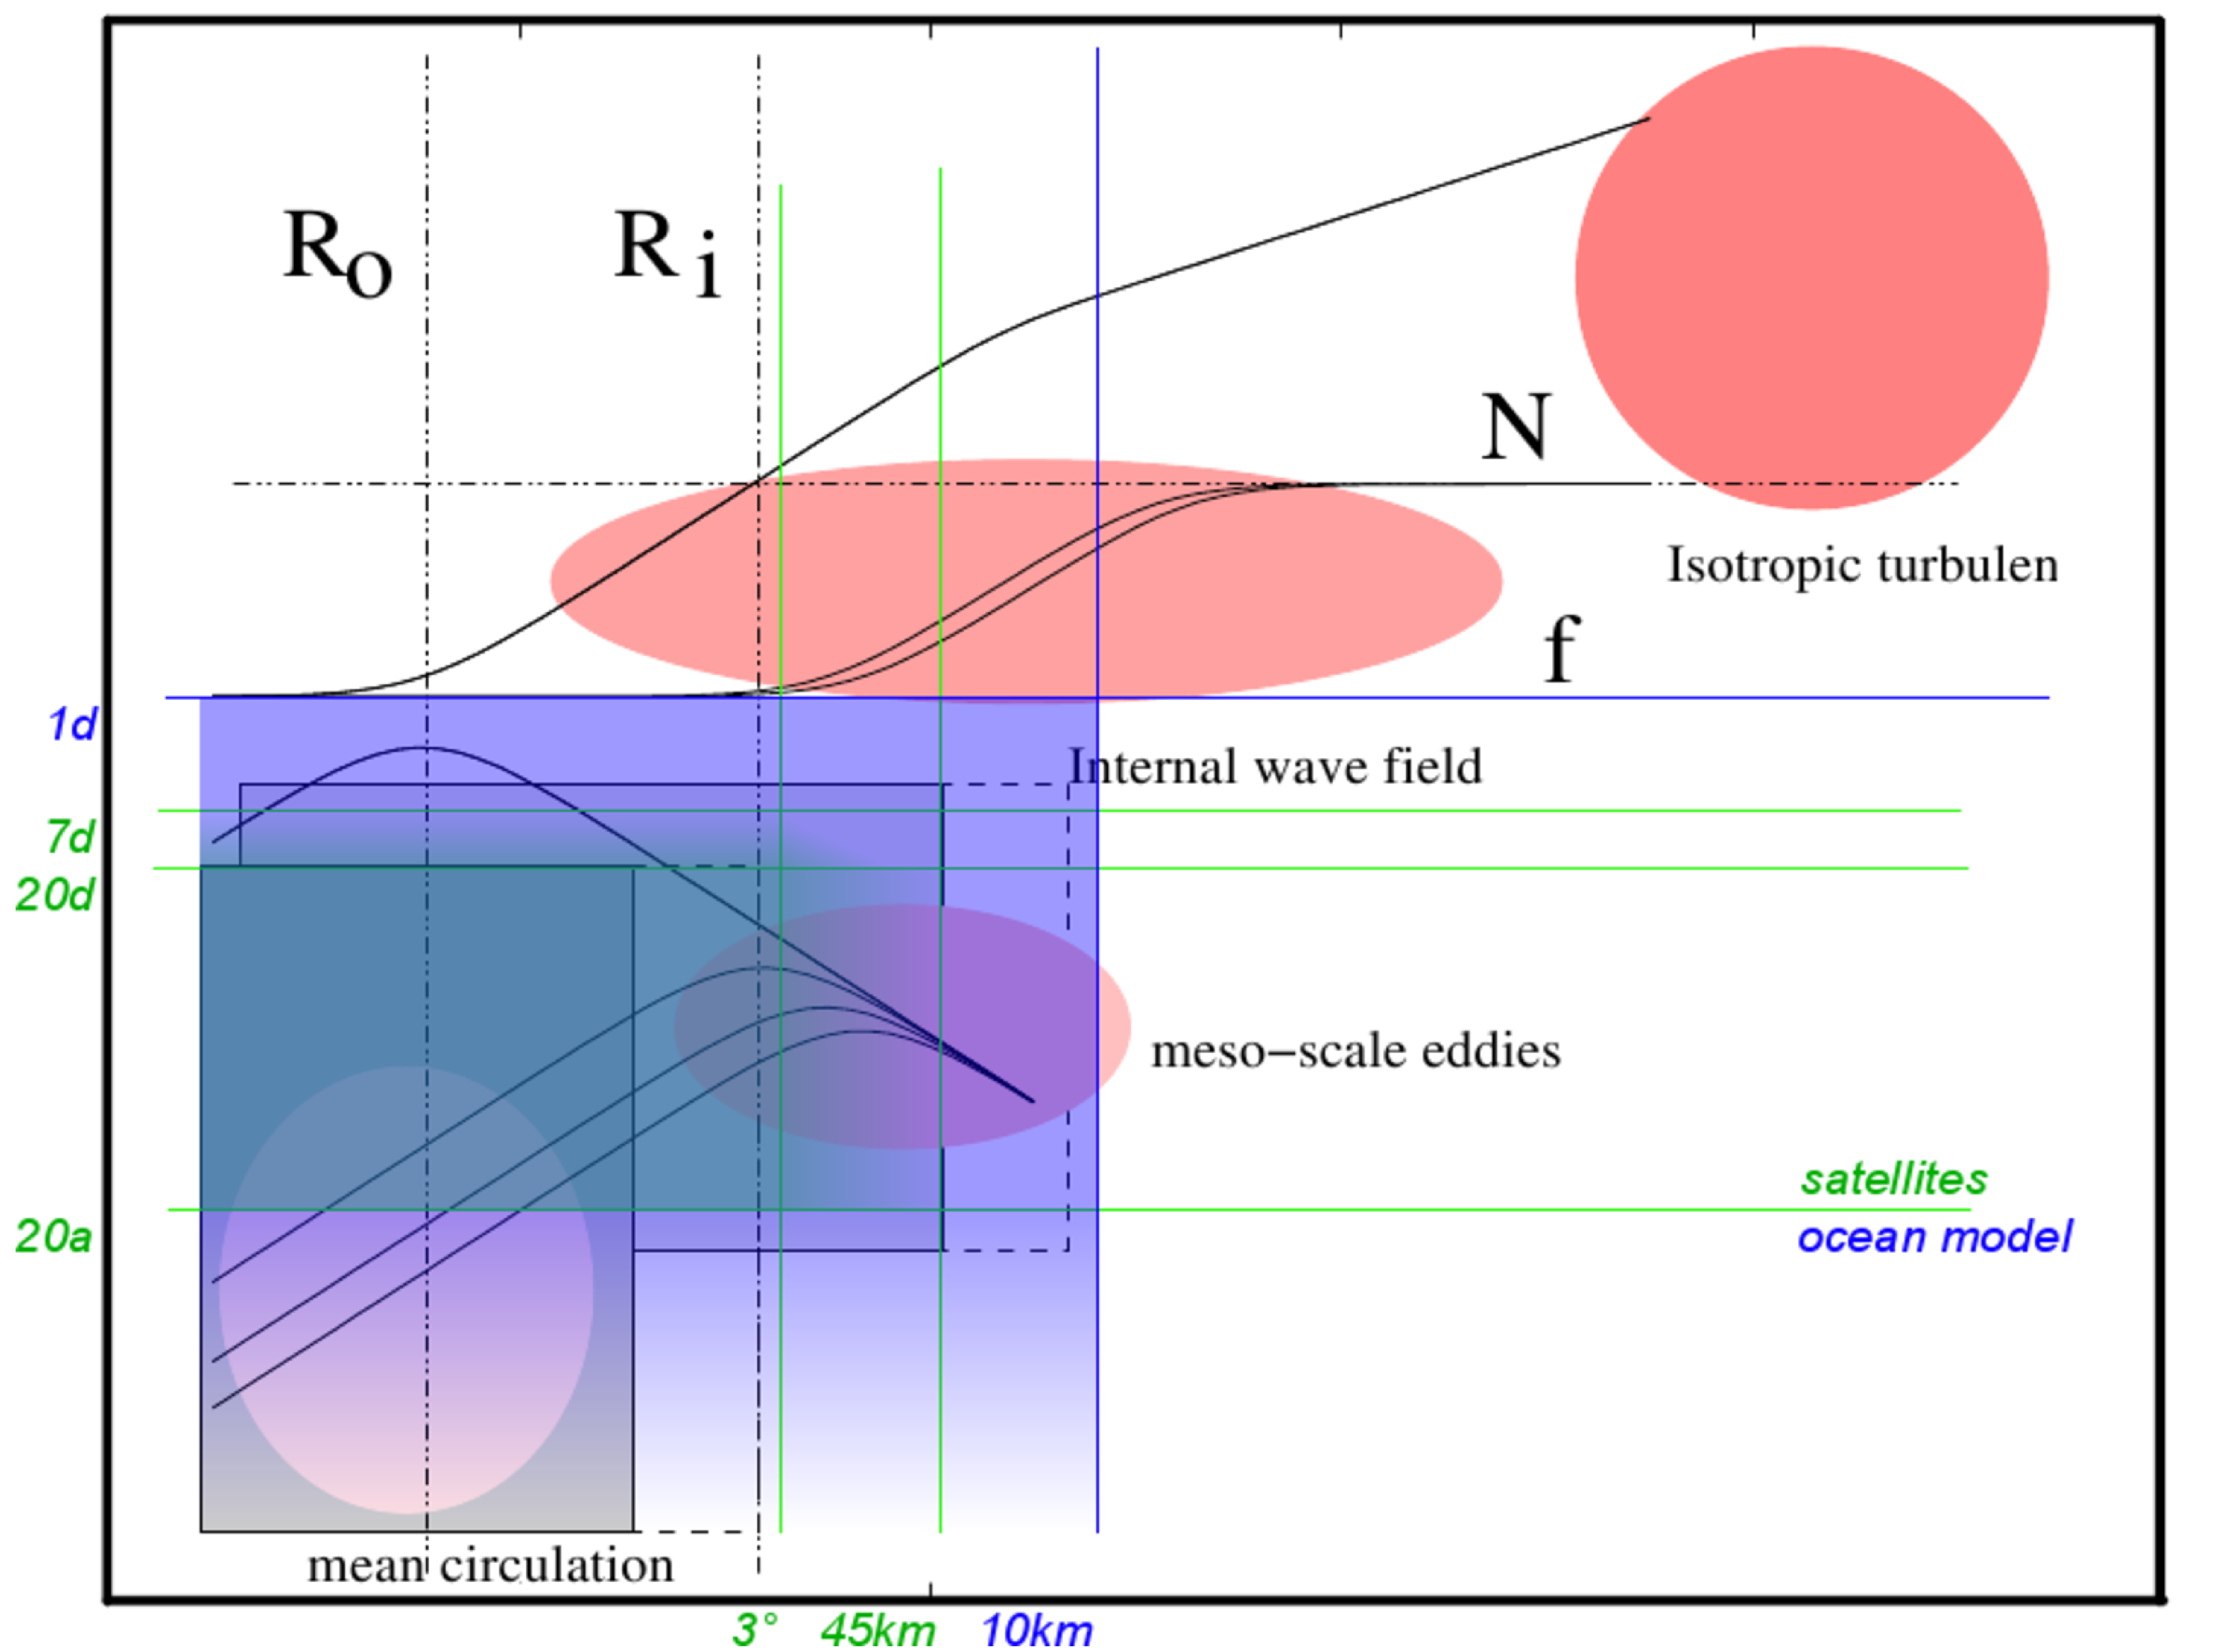
\includegraphics[width=.6\textwidth]{scales.pdf}
 \end{center}
 \vspace{-5mm}
\caption{Resolutions for model vs satellite. Modified version from \cite{olbers2012ocean}.}
\end{wrapfigure}


\begin{figure}[h]
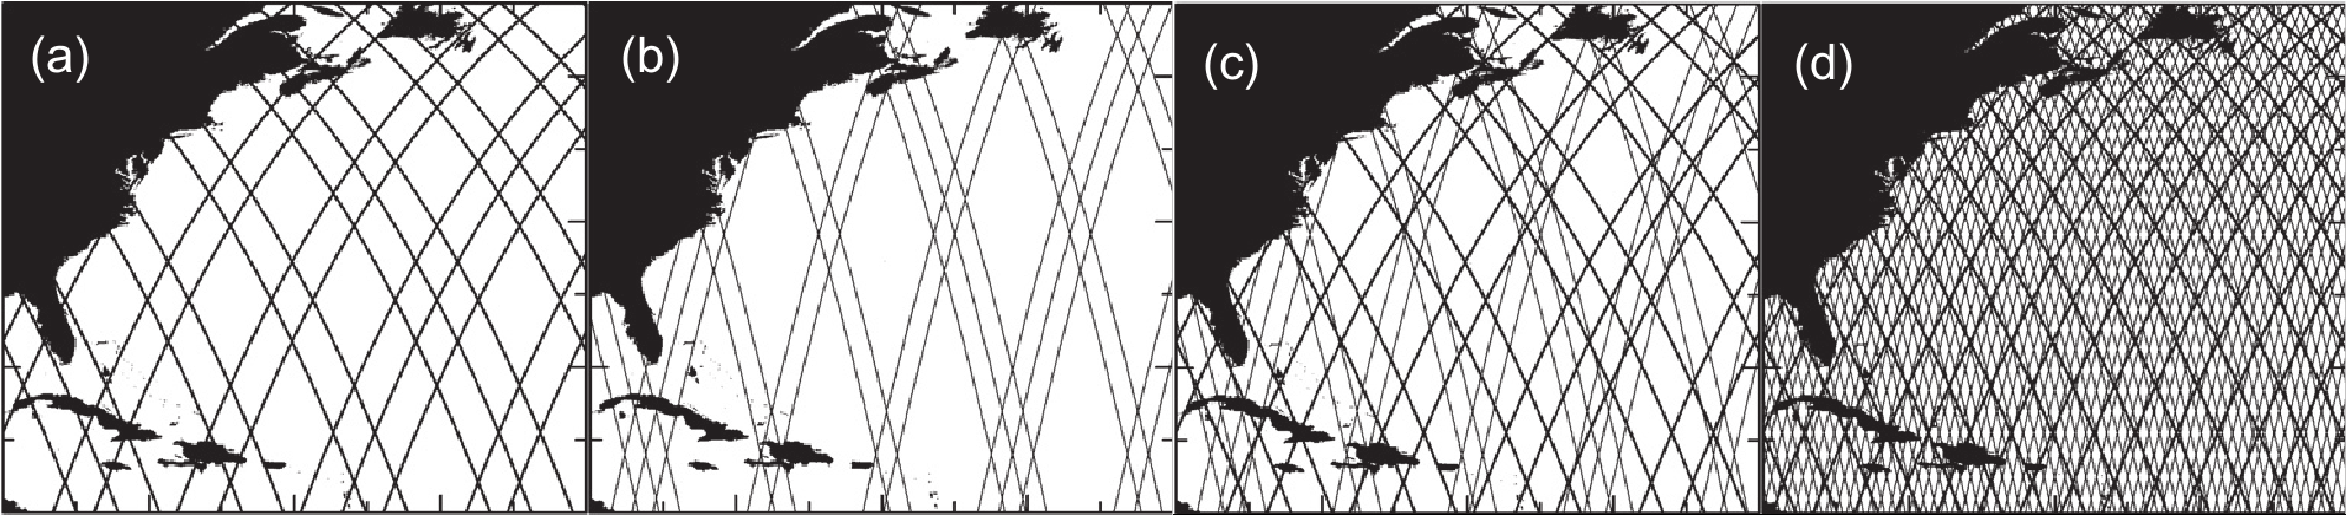
\includegraphics[width=\textwidth]{tracks.pdf}
\caption{{The ground track patterns for the 10-day repeat orbit of T/P and its successors Jason-1 and Jason-2 (thick lines) and the 35-day repeat orbit of ERS-1 and its successors ERS-2 and Envisat (thin lines). (a) The ground tracks of the 10-day orbit during a representative 7-day period; (b) The ground tracks of the 35-day orbit during the same representative 7-day period; (c) The combined ground tracks of the 10-day orbit and the 35-day orbit during the 7-day period; and (d) The combined ground tracks of the 10- day orbit and the 35-day orbit during the full 35 days of the 35-day orbit. (sic)} \cite{Chelton2011}}
\end{figure}


The merged ERS-1/Topex-data as used by \cite{Chelton2011} has a time step of 7 days. Assuming eddy drift speeds of $u_e=\order{-1}$m/s implies a distance traveled per time step of $L_{\delta t}\approx 60km$. \citeauthor{Chelton2011} estimate their effective spatial resolution as $\delta x \approx 40$km. Eddies of smaller scale are not resolved. Tracking a single eddy from one time-step to the next should hence be feasible, especially when $\vec{u}_e$ is approximately known. Problems arise when the sea level is characterized by an abundance of isolated vortices plus maybe even further meso-scale noise of comparable amplitude.
\begin{figure}
\begin{tabularx}{\textwidth}{ |X|X|X| }
  \hline
   & \bf{POP} & \bf{merged T/P - ERS-1 \footnote{the version used by \cite{Chelton2011}}}  \\
  \hline
  dx & $7km-11km$  & $1/3^{\circ}$ ($\approx 40 km$ after filtering)  \\
  \hline
  dt & $1d$  & $7d$  \\
  \hline
  $\log_{10}2$ filter cutoff & n/a  & $2^{\circ} $ by $ 2^{\circ} $  \\
  \hline
  z-levels & 42  & 1  \\
  \hline
  variables & SSH,S,T,u,v,w,tracers  & SSH  \\
  \hline
	pot. interpolation artifacts & n/a  & yes  \\
  \hline
	reality & no  & yes  \\
  \hline
\end{tabularx}
\end{figure}

Ambiguities arise in terms of correctly matching the eddies from the old time-step with those in the new one, potentially causing aliasing effects in the final
statistics. The translational speeds \footnote{$\order{1}$km/day} of eddies are not really the problem here, as they usually drift slow enough to not cover more
than 1 grid node per 7 day time step. The issue are those areas where eddies are born, die and merge. According to \cite{Smith2009} instabilities within the ACC
grow at rates of up to $1/(2 \mathrm{days})$, which means that at a time-step up to 3 eddies have emerged and equally many died for every eddy identified within
such region. The ground-repeat frequency of a satellite can of course not be set arbitrarily. Especially when the satellite is desired to cover as far north and
south as possible, whilst still being subjected to just the right torque from the earth's variable gravitational field to precess at preferably a
sun-synchronous frequency \ie $360^{\circ}/year$. Neither can the
satellite's altitude be chosen arbitrarily. If too low the oblateness of the earth creates too much eccentricity in the orbit that can no longer be
\textit{frozen} \footnote{minimizing undulating signals in altitude by choosing the right initial values.}. Another problem could be potential inhomogeneity in
the merged data in time dimension, since products of old and current missions are lumped together into one product. This is why \cite{Chelton2011} opted against
the finest resolution available and instead went for a product that had the most satellites merged in unison for the longest period of time.

\begin{figure}[h!]
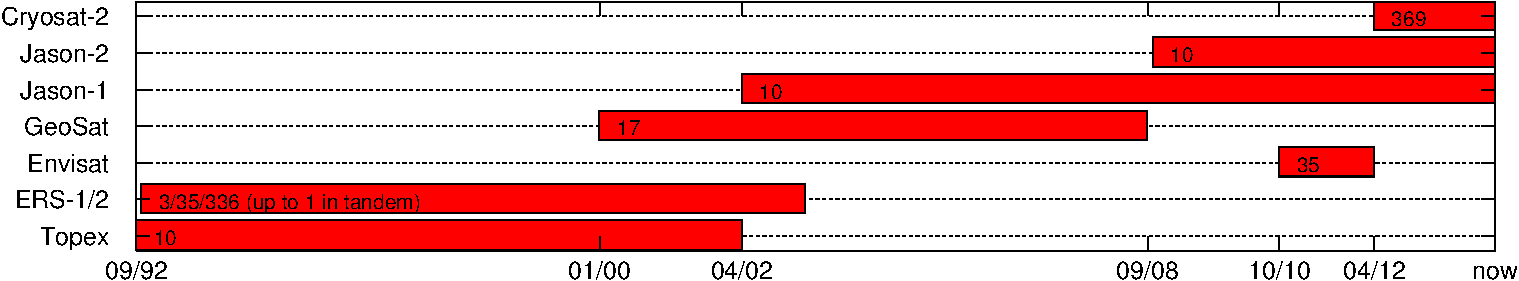
\includegraphics[width=\textwidth]{sats.pdf}
\caption{Length of mission. Numbers are orbit-period in days.}
\end{figure}


%%####################################################################
%%####################################################################

\paragraph{Ocean Model}


\begin{wrapfigure}[20]{r}{0.4\textwidth}
\vspace{-5mm}
  \begin{center}
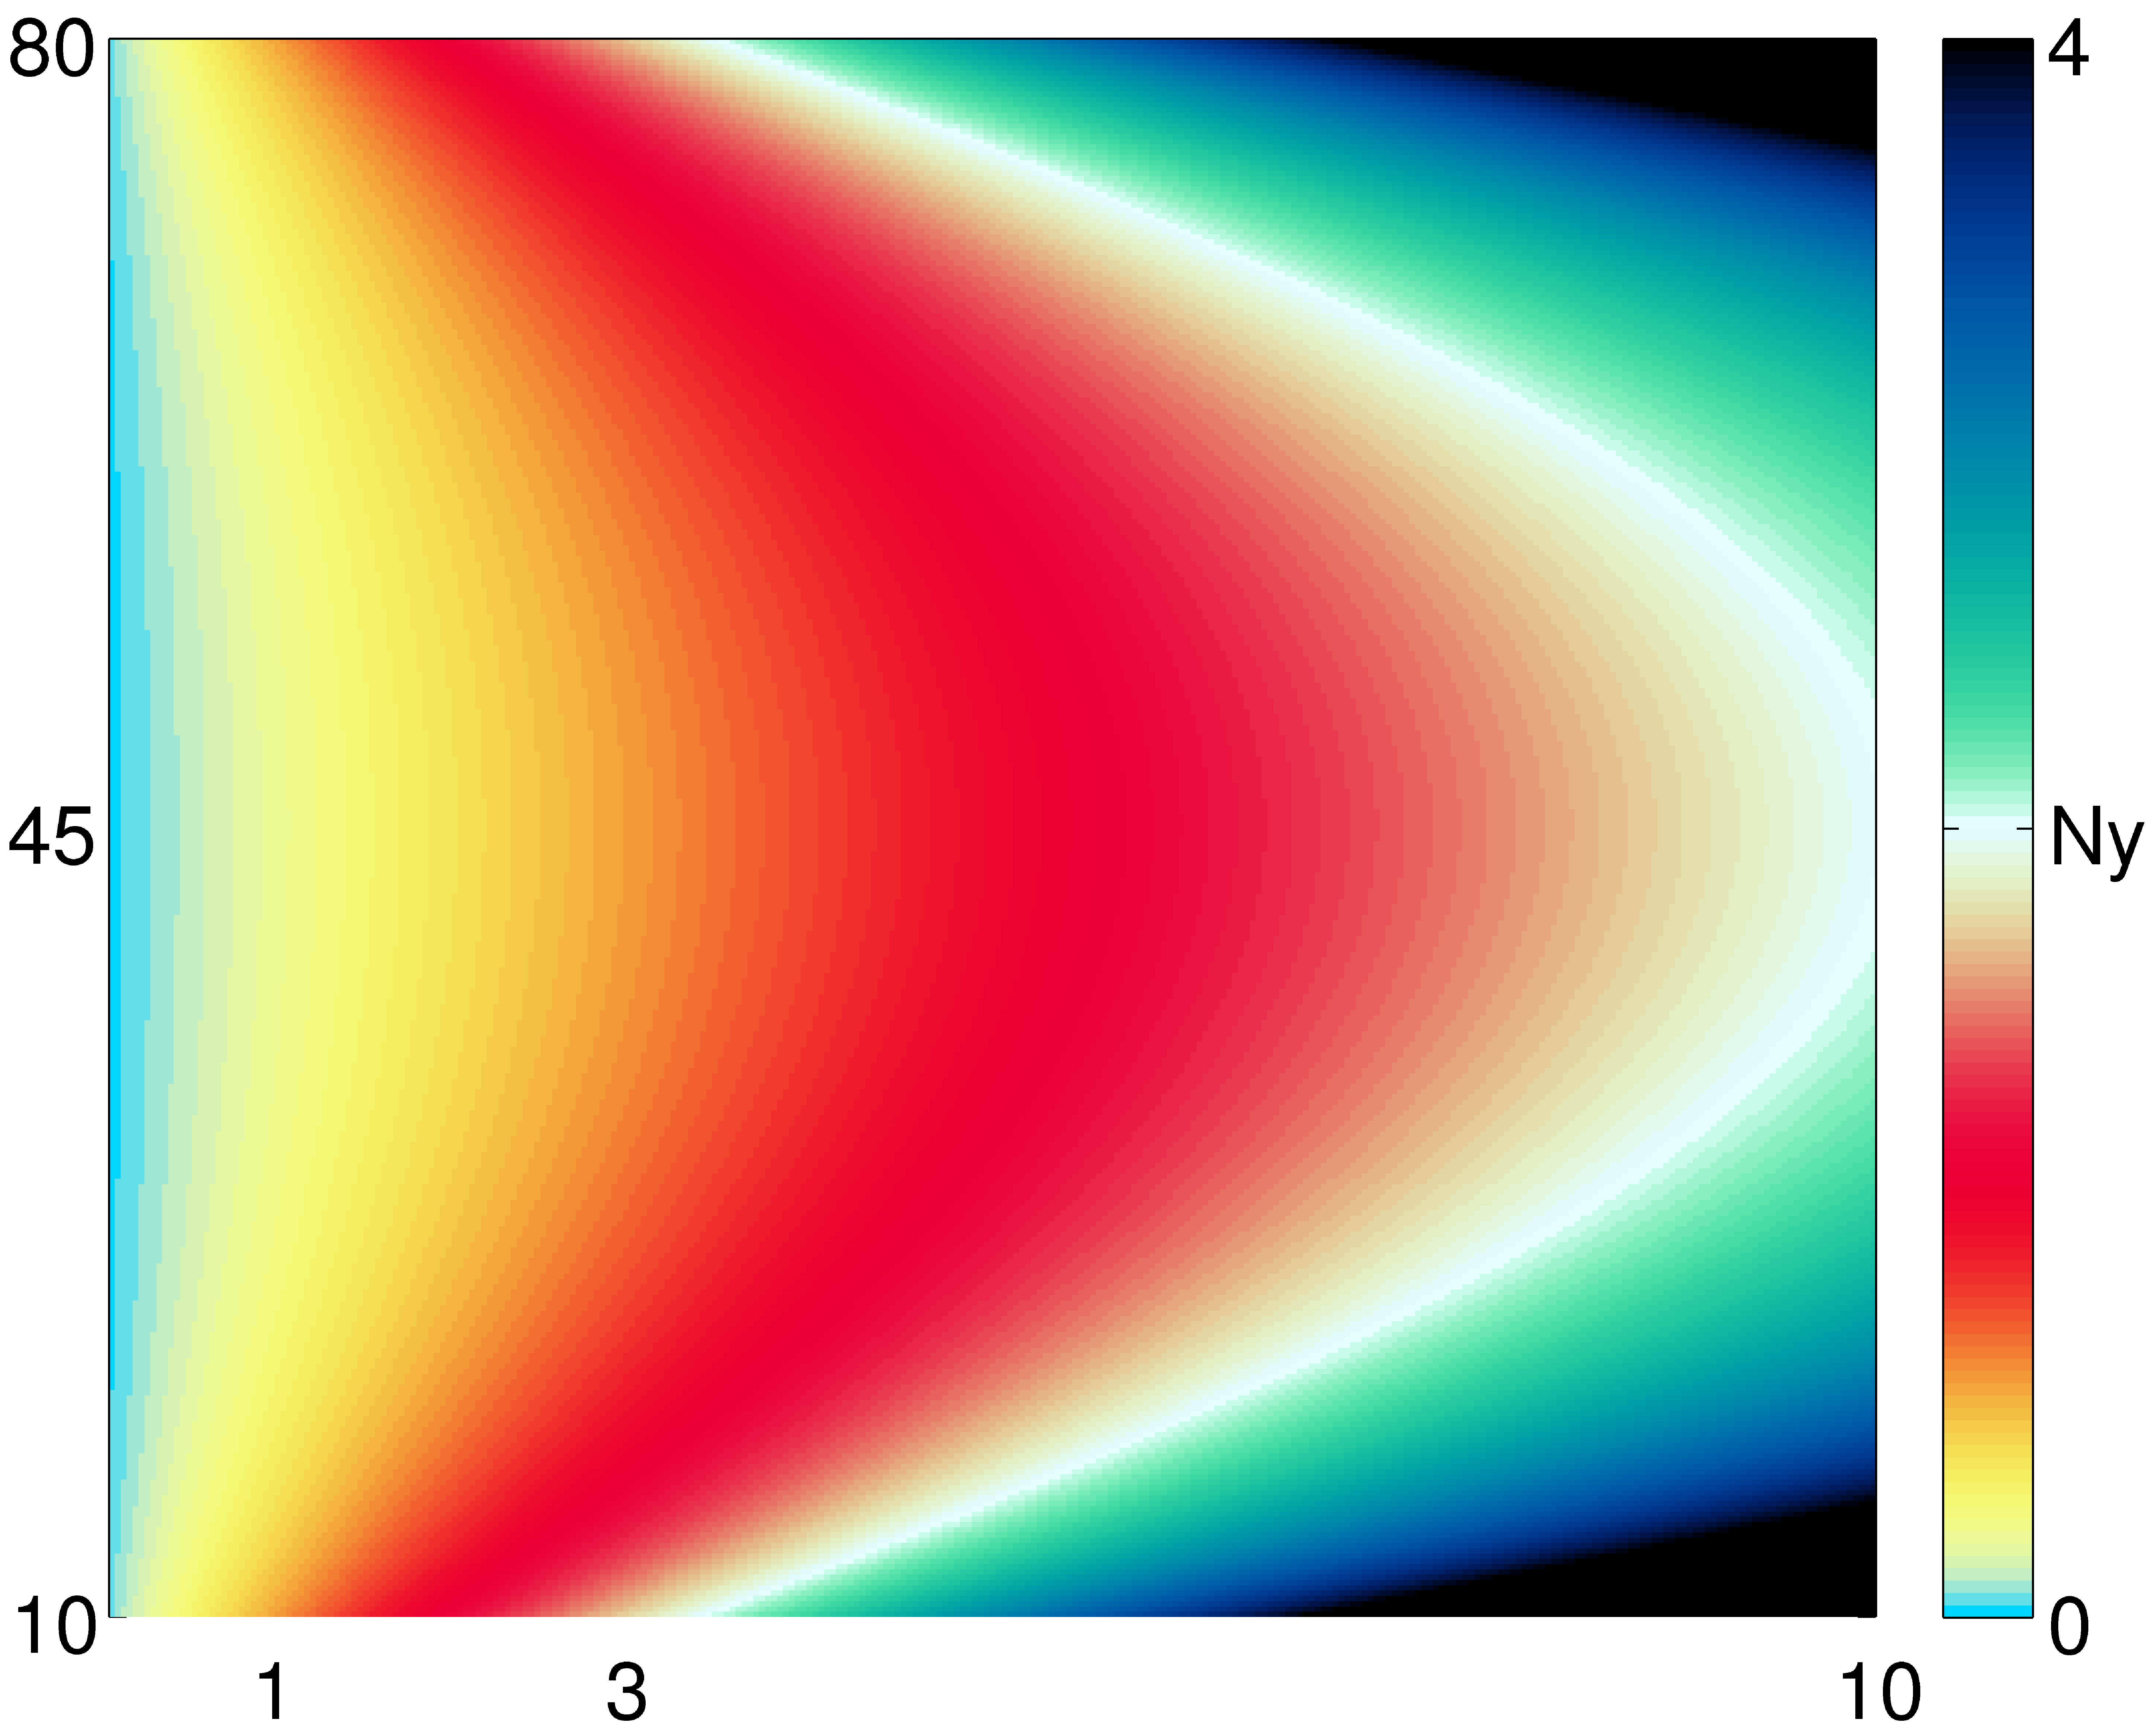
\includegraphics[width=.4\textwidth]{latovermu.pdf}
 \end{center}
  \vspace{-3mm}
\caption{$\xi(\phi,\mu)$. $\mathrm{Ny}\equiv 2$ \ie the Nyquist frequency.}\label{fig:phiovermu}
 %\vspace{-50mm}
\end{wrapfigure}
The advantages of detecting and tracking eddies from model data are obvious.
Say you have $\Bu=1$, so that $L=NH/f$. Let's assume \footnote{corresponds to $L(\phi=30^{\circ})=100$km} $NH=a/10d$, a model resolution of $1^{\circ}/\mu$ and that the eddy diameter was twice the Rossby radius. How many grid notes $\xi$ fit into one eddy as a function of latitude?
%%....................................................................
\begin{align}
	\xi \frac{a}{\mu} \frac{\cos \phi}{2 \pi}
	&=
	\frac{2NH }{f} = \frac{2NH 1d}{4 \pi  \sin(\phi)}\notag\\
	\xi
	&=
	 \frac{ 2\mu }{10  \sin(2\phi)}
\end{align}

See figure~\ref{fig:phiovermu} for the results. In this flat-bottom, constant $\rho_z$, Mercator-gridded model the worst eddy-resolution is interestingly at
mid-latitude. A value of $\xi>2$ is desirable, because it eradicates ambiguities in the tracking procedure, with the result that there is no need to
\textit{forecast} the position $x_e$ of an eddy for the new time step. It suffices to determine the closest eddy from the previous time-step for respective eddy
from the new time step and vice versa. Those 2 eddies that are in agreement are successfully matched, those from the new (old) time step that do not find a
match have just been born (have died). See also section \todoil{ref to section} for the technical stuff.
Another major advantage of the model is that it produces not only SSH data but also all other relevant variables \footnote{See section \ref{sec:goals} for all the
possibilities that arise.}, for not only the surface but for many different depths. The surface velocities inferred from altimetry are the geostrophic
components only, which should suffice to \eg determine the non-linearity and kinetic energy of an eddy for almost all regions, but less so for \eg the western
boundary currents.
The \emph{one} draw-back of using model data is that, in contrast to the satellite data, it does not represent reality.
\footnote{to be continued}

